% ============================================================================
% CHAPTER 5 --- NEURAL NETWORK-BASED SIMPLIFIED CLIPPING AND FILTERING (NN-SCF)
% ============================================================================
\chapter{Neural Network-Based Simplified Clipping and Filtering (NN-SCF)}
\label{ch:nnscf}

One of the primary techniques discussed in the first phase of this project is Clipping and Filtering (CF). It is arguably the most direct method for suppressing high PAPR in OFDM systems. However, classical Iterative Clipping and Filtering (ICF) algorithms suffer from a major operational bottleneck: they require repeated Fourier transforms to filter out-of-band distortion, which introduces severe computational latency. This chapter introduces the application of Deep Learning (DL) to enhance this framework, exploring how neural networks can entirely bypass these recursive transformations.

Specifically, we build upon the \textbf{Simplified Clipping and Filtering (SCF)} technique originally proposed by Wang and Tellambura~\cite{wang2005simplified}. We examine its deep learning counterpart, the \textbf{NN-SCF} architecture proposed by Sohn and Kim~\cite{sohn2015neural}. Rather than repeatedly shifting signals between the time and frequency domains, NN-SCF trains a pair of lightweight, sample-wise neural networks to instantly emulate the optimal noise-shaping behavior of classical SCF. This fundamentally eliminates the massive overhead of multiple Fast Fourier Transforms (FFTs), achieving near-identical PAPR reduction and Bit Error Rate (BER) performance with significantly lower latency.

% ============================================================================
\section{Simplified Clipping and Filtering (SCF)}
\label{sec:scf_principles}
% ============================================================================

Classical Clipping and Filtering (CF) suppresses high peak power by applying a hard threshold to the time-domain OFDM signal. However, this non-linear limiting operation generates out-of-band radiation and in-band distortion. Filtering the signal to suppress out-of-band leakage reconstructs the peak power, leading to the peak regrowth phenomenon.

To mitigate peak regrowth, classical Iterative Clipping and Filtering (ICF) repeats the clipping and filtering steps recursively. While effective, executing $L$ iterations of ICF requires $2L+1$ Fourier transform operations (FFTs/IFFTs), introducing significant latency and computational complexity.

\subsection{Mathematical Model of SCF}

The Simplified Clipping and Filtering (SCF) technique~\cite{wang2005simplified} prevents peak regrowth in a single iteration. Rather than repeatedly transforming the signal between domains, SCF simply clips the time-domain signal once, extracts the clipping noise, and subtracts a filtered version of it directly from the original frequency-domain data.

For an oversampled time-domain OFDM signal $x_n = x_I(n) + j x_Q(n)$, the amplitude-clipped signal $\hat{x}_n$ is defined as:
\begin{equation*}
    \hat{x}_n = \begin{cases}
        x_n,              & |x_n| \le A \\
        A e^{j \theta_n}, & |x_n| > A
    \end{cases}
\end{equation*}
where $A$ represents the predefined clipping amplitude threshold, and $\theta_n = \arg(x_n)$ represents the phase of the original signal sample. The threshold $A$ is determined by the Clipping Ratio (CR), which is defined relative to the root-mean-square (RMS) level of the signal $\sigma$:
\begin{equation*}
    \mathrm{CR} = \frac{A}{\sigma}
\end{equation*}

The clipping noise $f_n$, which captures the signal distortion introduced by the thresholding operation, is isolated in the time domain:
\begin{equation*}
    f_n = x_n - \hat{x}_n = \begin{cases}
        0,                      & |x_n| \le A \\
        x_n - A e^{j \theta_n}, & |x_n| > A
    \end{cases}
\end{equation*}
This time-domain noise sequence is sparse, containing non-zero elements only at samples where the amplitude exceeded the threshold $A$. To filter the out-of-band noise, $f_n$ is converted to the frequency domain via a Fast Fourier Transform (FFT):
\begin{equation*}
    F_k = \mathrm{FFT}\{f_n\}.
\end{equation*}
The out-of-band noise components are then zeroed, while the in-band noise components on active subcarriers are preserved, yielding the filtered noise spectrum $\tilde{F}_k$:
\begin{equation*}
    \tilde{F}_k = \begin{cases}
        F_k, & \text{for active subcarriers}      \\
        0,   & \text{for out-of-band subcarriers}
    \end{cases}
\end{equation*}

\subsection{Bussgang's Theorem and the Scaling Coefficient}

The key innovation of the SCF technique lies in the frequency-domain reconstruction. According to \textbf{Bussgang's Theorem}, the output of a memoryless non-linear device driven by a Gaussian input (which closely models an OFDM signal with a large number of subcarriers) can be represented as a scaled version of the input signal plus an uncorrelated distortion component.

By modeling the iterative convergence of ICF, Wang and Tellambura~\cite{wang2005simplified} derived a closed-form scaling coefficient $\bar{\beta}$ to scale the filtered clipping noise $\tilde{F}_k$ before subtraction. The final SCF output in the frequency domain is expressed as:
\begin{equation*}
    \bar{X}_k = X_k - \bar{\beta} \tilde{F}_k
\end{equation*}
where $X_k$ represents the original frequency-domain subcarrier symbols. The scaling factor $\bar{\beta}$ analytically emulates the cumulative noise-attenuation effect of $k$ virtual iterations of ICF, and is defined as:
\begin{equation*}
    \bar{\beta} = \frac{1 - (1 - \bar{\alpha})^{3k/2}}{1 - (1 - \bar{\alpha})^{3/2}}
\end{equation*}
Here, $\bar{\alpha}$ is the auxiliary attenuation parameter that quantifies the clipping severity, assuming complex Gaussian statistics for the time-domain samples:
\begin{equation*}
    \bar{\alpha} = \frac{2\sqrt{2}}{\sqrt{3\pi}} \frac{\sigma}{A}
\end{equation*}
where $\sigma$ is the standard deviation of the complex Gaussian process. Finally, the time-domain SCF signal is obtained by taking the Inverse Fast Fourier Transform (IFFT):
\begin{equation*}
    \bar{x}_n = \mathrm{IFFT}\{\bar{X}_k\}.
\end{equation*}

\begin{figure}[H]
    \centering
    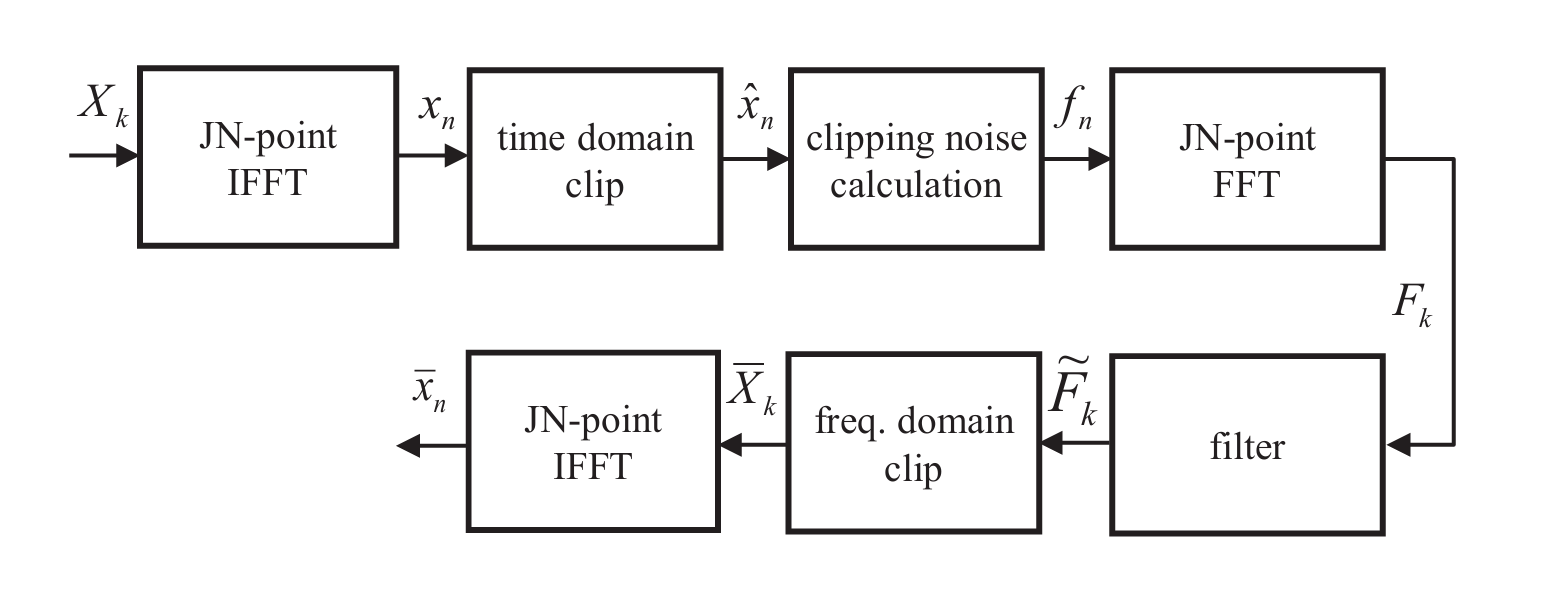
\includegraphics[width=0.9\linewidth]{Figures/NN_SCF/scf_block_diagram.png}
    \caption{Block diagram of the classical Simplified Clipping and Filtering (SCF) algorithm~\cite{sohn2015neural}. The technique requires three separate Fourier transform operations: an initial IFFT to generate the time-domain signal, an FFT to extract the frequency-domain clipping noise, and a final IFFT to reconstruct the filtered time-domain signal.}
    \label{fig:scf_block_diagram}
\end{figure}

As shown in Figure~\ref{fig:scf_block_diagram}, although SCF avoids multiple iterations, it still requires \textbf{three Fourier transforms} per block (one initial IFFT to obtain $x_n$, one FFT to obtain $F_k$, and one final IFFT to obtain $\bar{x}_n$). Since the complexity of each transform scales as $\mathcal{O}(N \log_2 N)$, the computational bottleneck remains substantial, especially for large subcarrier counts.

% ============================================================================
\section{Neural Network-Based PAPR Reduction (NN-SCF)}
\label{sec:nnscf_framework}
% ============================================================================

To eliminate the computational burden of additional Fourier transforms, Sohn and Kim~\cite{sohn2015neural} proposed replacing the classical SCF algorithm with an \textbf{Artificial Neural Network (ANN)} mapper.

The core idea of \textbf{NN-SCF} is to train a neural network offline to directly map the original time-domain signal $x_n$ to its low-PAPR output $\bar{x}_n$. During online inference, the network processes the signal sample-by-sample entirely in the time domain, successfully bypassing all explicit clipping, noise filtering, and extra FFT operations.

\subsection{Parallel Real-Valued MLP Architecture}

Because standard neural network frameworks operate on real numbers, processing the complex-valued time-domain OFDM signal $x_n = x_I(n) + j x_Q(n)$ requires special architectural design. Rather than utilizing complex-valued backpropagation, NN-SCF employs two independent, parallel real-valued Multi-Layer Perceptrons (MLPs):
\begin{itemize}
    \item $\mathrm{ModNN}_{\mathrm{Re}}$: Approximates the real (in-phase) transformation $x_I(n) \to \bar{x}_I(n)$.
    \item $\mathrm{ModNN}_{\mathrm{Im}}$: Approximates the imaginary (quadrature) transformation $x_Q(n) \to \bar{x}_Q(n)$.
\end{itemize}

Each network is designed with a highly compact, sample-wise topology to minimize inference complexity:
\begin{enumerate}
    \item \textbf{Input Layer}: Contains $1$ neuron, which receives a single normalized real-valued sample $x$ (representing either $x_I(n)$ or $x_Q(n)$).
    \item \textbf{Hidden Layer 1}: Contains $2$ neurons. It applies a weight matrix $W_1$ and bias vector $b_1$, followed by a non-linear activation function.
    \item \textbf{Hidden Layer 2}: Contains $1$ neuron. It applies weight vector $W_2$ and bias $b_2$, followed by the activation function.
    \item \textbf{Output Layer}: Contains $1$ neuron, utilizing a linear activation function (weights $W_3$, bias $b_3$) to yield the reconstructed sample.
\end{enumerate}

To match the peak-limiting characteristics of clipping, the hidden layers employ a custom \textbf{triangular activation function} $\phi(z)$ (equivalent to MATLAB's \texttt{tribas}):
\begin{equation*}
    \phi(z) = \max(1 - |z|,\, 0)
\end{equation*}
Mathematically, the forward pass of the network is formulated as:
\begin{align*}
    h_1     & = \phi(W_1 x + b_1)   \\
    h_2     & = \phi(W_2 h_1 + b_2) \\
    \hat{y} & = W_3 h_2 + b_3
\end{align*}
where $W_i$ and $b_i$ represent the weights and biases of the respective layers, and $\hat{y}$ is the output of the network (approximating $\bar{x}_I(n)$ or $\bar{x}_Q(n)$). The bounded nature of the triangular function is highly suited to peak-limiting regressions, allowing the model to converge rapidly with very few neurons. The output of the parallel network is combined to reconstruct the complex time-domain signal:
\begin{equation*}
    \bar{x}_n = \mathrm{ModNN}_{\mathrm{Re}}\{x_I(n)\} + j \mathrm{ModNN}_{\mathrm{Im}}\{x_Q(n)\}
\end{equation*}

\subsection{Computational Complexity Comparison}

The primary benefit of the NN-SCF mapper is the dramatic reduction in computational complexity. In the online transmission phase, the system requires only a single initial IFFT to generate $x_n$ from the subcarrier symbols $X_k$. The clipping and filtering noise compensation is then performed sample-by-sample by the parallel MLPs.

For $N$ subcarriers, the mathematical complexity of a standard $N$-point FFT is modeled as $\frac{N}{2} \log_2 N$ complex multiplications and $N \log_2 N$ complex additions. For the $1\text{--}2\text{--}1\text{--}1$ neural network, the forward pass of a single sample requires only $5$ real multiplications and $5$ real additions. With two networks operating in parallel, the total neural network overhead is $10N$ real multiplications and $10N$ real additions per OFDM block.

Table~\ref{tab:scf_complexity} presents a comprehensive complexity comparison between classical ICF, SCF, Selective Mapping (SLM), and the proposed NN-SCF scheme.

\begin{table}[H]
    \centering
    \caption{Computational complexity comparison per OFDM block for $N = 256$ subcarriers, $L = 3$ ICF iterations, and $U = 16$ SLM candidate blocks~\cite{sohn2015neural}.}
    \label{tab:scf_complexity}
    \begin{tabular}{l c c c c}
        \toprule
        \textbf{Operation / Complexity} & \textbf{ICF ($L=3$)} & \textbf{SCF} & \textbf{SLM ($U=16$)} & \textbf{Proposed NN-SCF} \\
        \midrule
        (I)FFT operations               & $7$                  & $3$          & $16$                  & $1$                      \\
        Complex Multiplications         & $7{,}168$            & $3{,}072$    & $16{,}384$            & $1{,}024$                \\
        Complex Additions               & $14{,}336$           & $6{,}144$    & $32{,}768$            & $2{,}048$                \\
        Real Multiplications (NN)       & —                    & —            & —                     & $2{,}560$                \\
        Real Additions (NN)             & —                    & —            & —                     & $2{,}560$                \\
        Clip Operations                 & $1$                  & $2$          & —                     & $0$                      \\
        Check Operations                & —                    & —            & $16$                  & $0$                      \\
        \bottomrule
    \end{tabular}
\end{table}

As shown in Table~\ref{tab:scf_complexity}, the proposed NN-SCF scheme reduces the number of expensive Fourier transforms by $7\times$ compared to ICF and $3\times$ compared to classical SCF. The bulk of the remaining calculations are converted from complex arithmetic to highly parallelizable, low-cost real additions and multiplications.

% ============================================================================
\section{System Implementation}
\label{sec:nnscf_implementation}
% ============================================================================

To validate the theoretical advantages of the NN-SCF mapper, a simulation pipeline was developed using Python, NumPy, and PyTorch. The simulation environment parameters were configured to replicate the standard benchmarks used in the literature, as detailed in Table~\ref{tab:scf_parameters}.

\begin{table}[H]
    \centering
    \caption{Simulation and system parameters for the NN-SCF pipeline.}
    \label{tab:scf_parameters}
    \begin{tabular}{l r}
        \toprule
        \textbf{Parameter}                      & \textbf{Value}                       \\
        \midrule
        Subcarriers ($N$)                       & $256$                                \\
        Oversampling Factor ($J$)               & $4 \implies N_{\mathrm{fft}} = 1024$ \\
        Cyclic Prefix (CP) Length               & $64$                                 \\
        Clipping Ratio (CR)                     & $6$ dB                               \\
        ICF Iterations ($L$) / SCF Target ($k$) & $3$                                  \\
        Modulation Schemes                      & QPSK, $16$-QAM                       \\
        Data Batch Size                         & $10{,}000$ symbols                   \\
        \bottomrule
    \end{tabular}
\end{table}

\subsection{Dataset Generation and Normalization}

The dataset was generated by transmitting random bitstreams modulated under QPSK or 16-QAM schemes. Oversampling with a factor of $J = 4$ was enforced by padding the frequency-domain symbol vector with $768$ guard subcarriers before taking the $1024$-point IFFT. This is physically necessary because Nyquist-rate sampling ($J=1$) underestimates the analog peaks and ignores peak regrowth.

The generated time-domain signal $x_n$ served as the training input. The target (ground truth) was obtained by passing $x_n$ through the classical SCF algorithm with $k=3$ virtual iterations. Both the inputs and targets were split into real and imaginary components.

To accelerate backpropagation and match the bounded range of the triangular activation function, the real and imaginary components were normalized to the range $[-1, +1]$ using Min-Max scaling:
\begin{equation*}
    X_{\mathrm{norm}} = 2 \cdot \frac{X_{\mathrm{raw}} - X_{\mathrm{min}}}{X_{\mathrm{max}} - X_{\mathrm{min}}} - 1
\end{equation*}
where $X_{\mathrm{min}}$ and $X_{\mathrm{max}}$ were computed across the training batch and saved as metadata to perform exact physical reconstruction during testing:
\begin{equation*}
    Y_{\mathrm{pred}} = \left(\frac{Y_{\mathrm{pred, norm}} + 1}{2}\right)(Y_{\mathrm{max}} - Y_{\mathrm{min}}) + Y_{\mathrm{min}}
\end{equation*}

\subsection{Neural Network Training Details}

The custom PyTorch model implements the $1\text{--}2\text{--}1\text{--}1$ topology described in Section~\ref{sec:nnscf_framework}.

While the original paper~\cite{sohn2015neural} recommends the Levenberg-Marquardt optimizer, standard deep learning libraries like PyTorch lack native, efficient support for second-order Marquardt optimization on large datasets. Consequently, we utilized the \textbf{Adam optimizer} with a learning rate of $0.001$. The networks were trained independently to minimize the Mean Squared Error (MSE) loss:
\begin{equation*}
    \mathcal{L}_{\mathrm{MSE}} = \frac{1}{N_{tr}} \sum_{i=1}^{N_{tr}} (y_i - \hat{y}_i)^2
\end{equation*}
Both networks were trained for $100$ epochs using $70$ training packages, with validation loss monitored on $10$ validation packages at the end of each epoch to prevent overfitting.

% ============================================================================
\section{Simulation Results and Analysis}
\label{sec:nnscf_results}
% ============================================================================

After training, the saved PyTorch model weights were loaded to evaluate the model's inference performance on the remaining $20$ testing packages.

\subsection{Cubic Metric (CM) Performance}

The Cubic Metric (CM) represents the power envelope fluctuations of the OFDM signal more accurately than PAPR when designing power amplifiers, as it accounts for the cubic non-linearities of the active components. The raw cubic metric (RCM) is defined as:
\begin{equation*}
    \mathrm{RCM} = 20\log_{10}\left(\mathrm{rms}\left[\left(\frac{|x_n|}{\mathrm{rms}(x_n)}\right)^3\right]\right)
\end{equation*}
The standard CM in decibels is calculated relative to a reference signal:
\begin{equation*}
    \mathrm{CM} = \frac{\mathrm{RCM} - \mathrm{RCM}_{\mathrm{ref}}}{K}
\end{equation*}
where $\mathrm{RCM}_{\mathrm{ref}} = 1.52$ dB represents the RCM of a reference WCDMA signal, and $K = 1.56$ is an empirical scaling factor~\cite{sohn2015neural}.

\begin{figure}[H]
    \centering
    \begin{subfigure}[b]{0.48\textwidth}
        \centering
        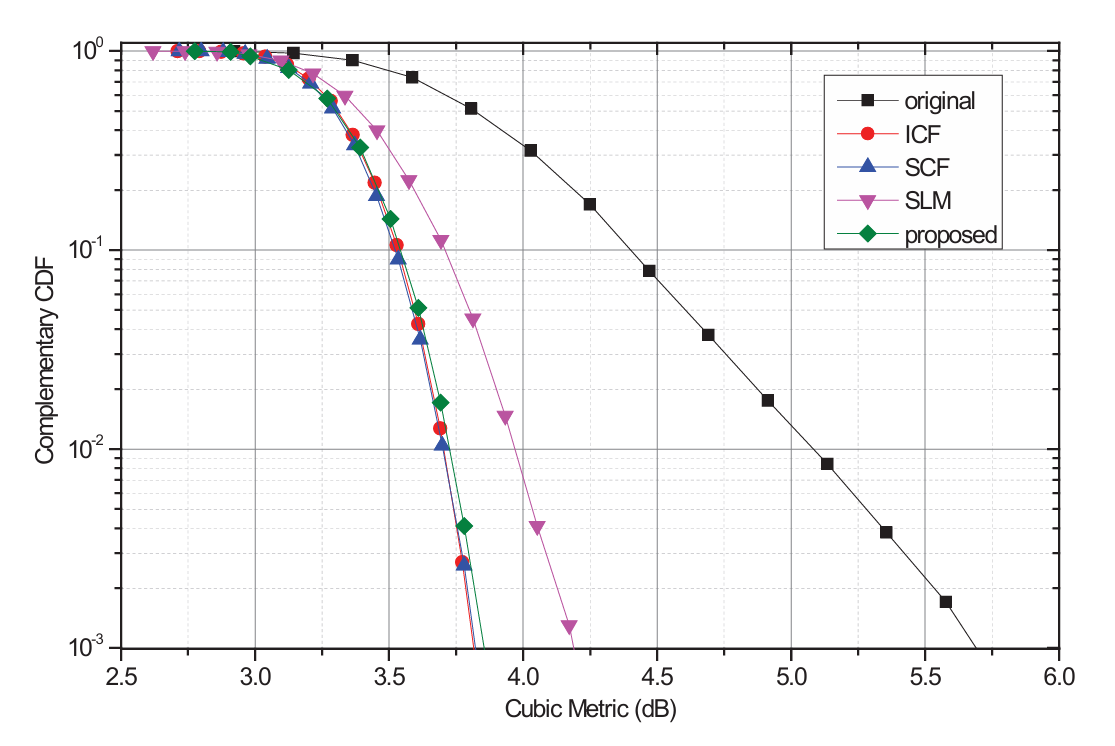
\includegraphics[width=\textwidth]{Figures/NN_SCF/cm_qpsk_paper.png}
        \caption{Results from the original paper~\cite{sohn2015neural}}
        \label{fig:cm_qpsk_paper}
    \end{subfigure}
    \hfill
    \begin{subfigure}[b]{0.48\textwidth}
        \centering
        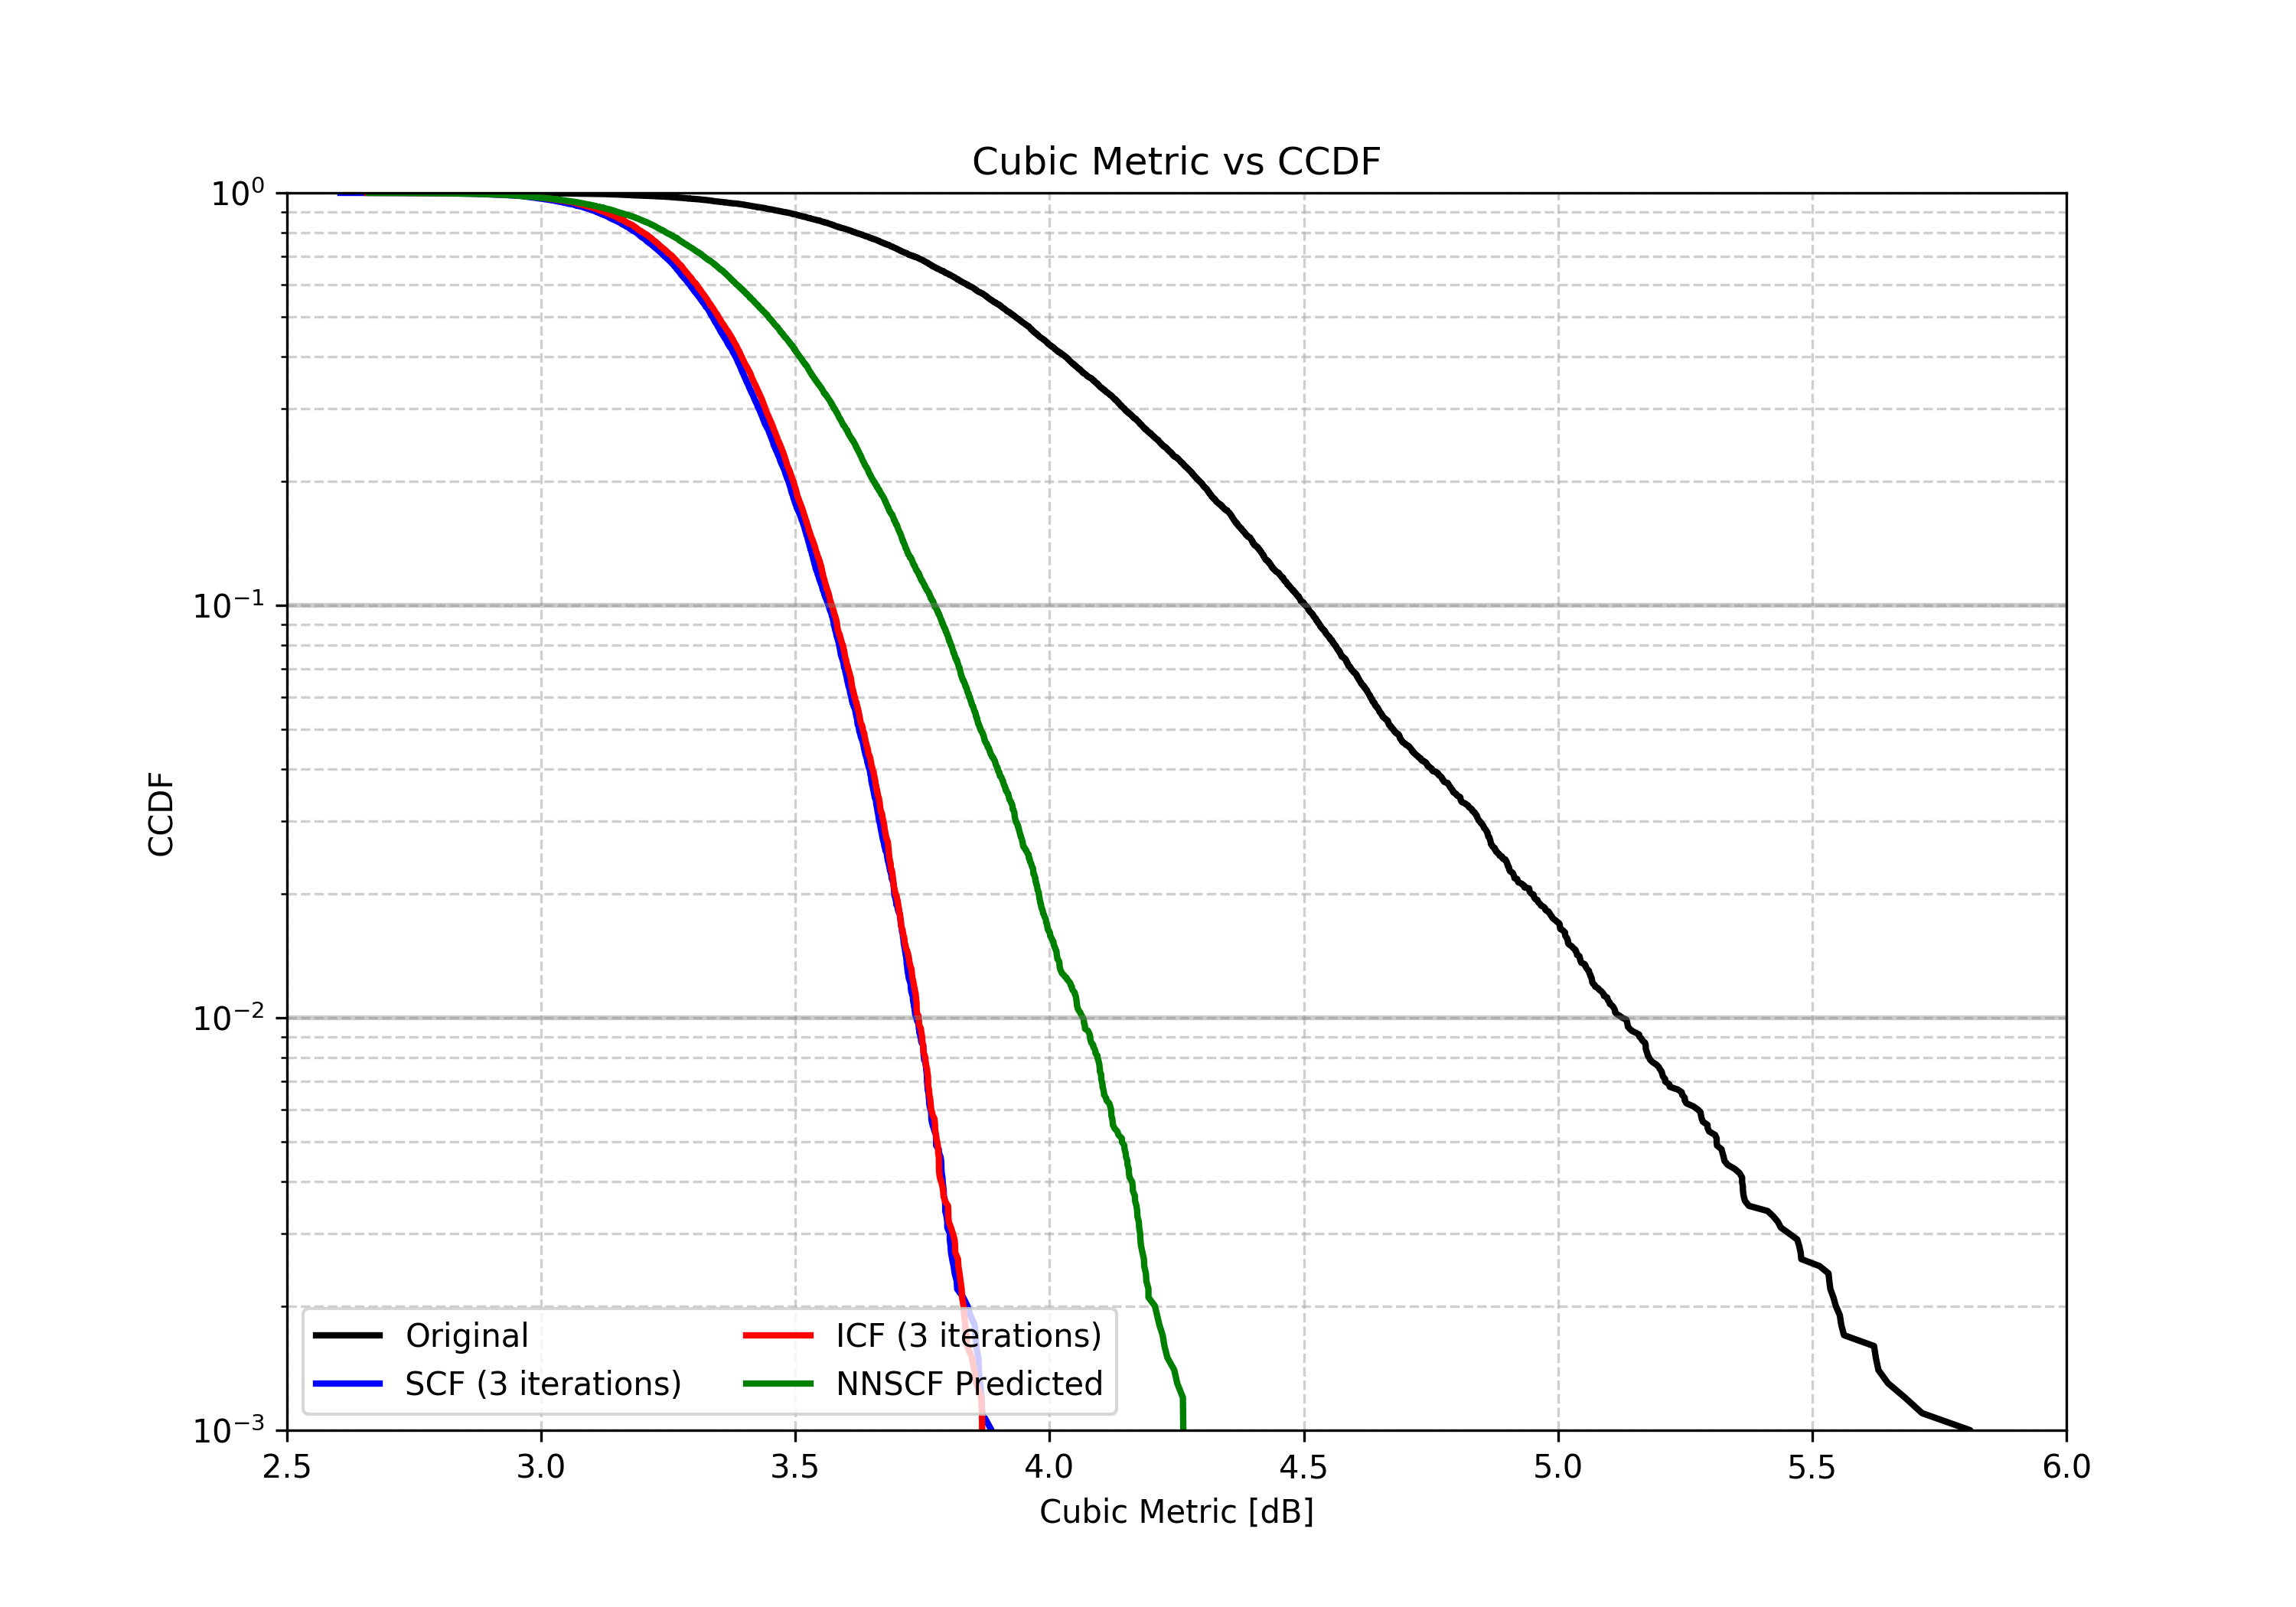
\includegraphics[width=0.96\textwidth]{Figures/NN_SCF/cm_qpsk_reproduced.png}
        \caption{Our simulated results}
        \label{fig:cm_qpsk_reproduced}
    \end{subfigure}
    \caption{CCDF of the Cubic Metric (CM) for QPSK modulated OFDM signals ($N=256$), comparing (a) original results~\cite{sohn2015neural} and (b) our PyTorch reproduction. The plot evaluates the capacity of the NN-SCF mapper to reproduce classical SCF noise compensation.}
    \label{fig:cm_qpsk_comparison}
\end{figure}

Figure~\ref{fig:cm_qpsk_comparison} compares the Complementary Cumulative Distribution Function (CCDF) of the Cubic Metric for QPSK modulation. Our PyTorch implementation successfully reproduces the curves reported by the original authors. The NN-SCF curves lie within $0.1$ dB of the classical SCF baseline at a CCDF of $10^{-3}$, representing a significant $1.3$ dB reduction in envelope fluctuation compared to original OFDM. This confirms that the lightweight neural network has accurately captured the complex, non-linear clipping noise cancellation.

\subsection{Bit Error Rate (BER) Performance}

Next, the Bit Error Rate (BER) performance was simulated over an Additive White Gaussian Noise (AWGN) channel to evaluate signal reconstruction accuracy.

\begin{figure}[H]
    \centering
    \begin{subfigure}[b]{0.48\textwidth}
        \centering
        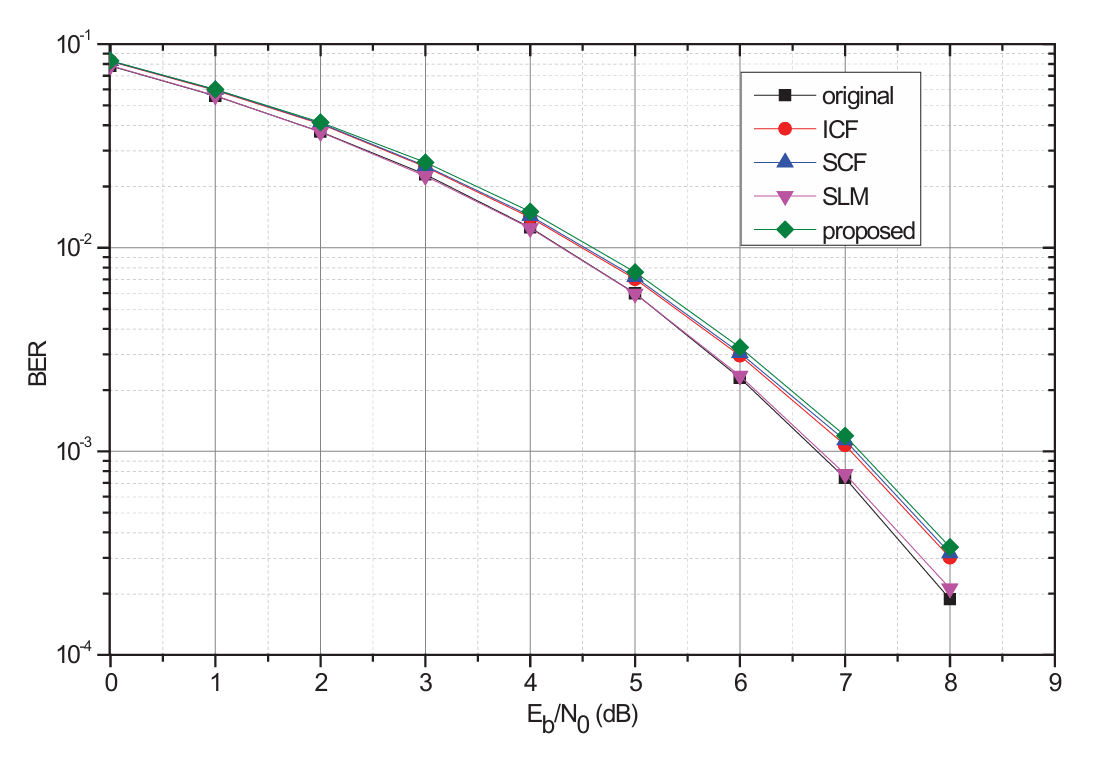
\includegraphics[width=\textwidth]{Figures/NN_SCF/ber_qpsk_paper.png}
        \caption{Results from the original paper~\cite{sohn2015neural}}
        \label{fig:ber_qpsk_paper}
    \end{subfigure}
    \hfill
    \begin{subfigure}[b]{0.48\textwidth}
        \centering
        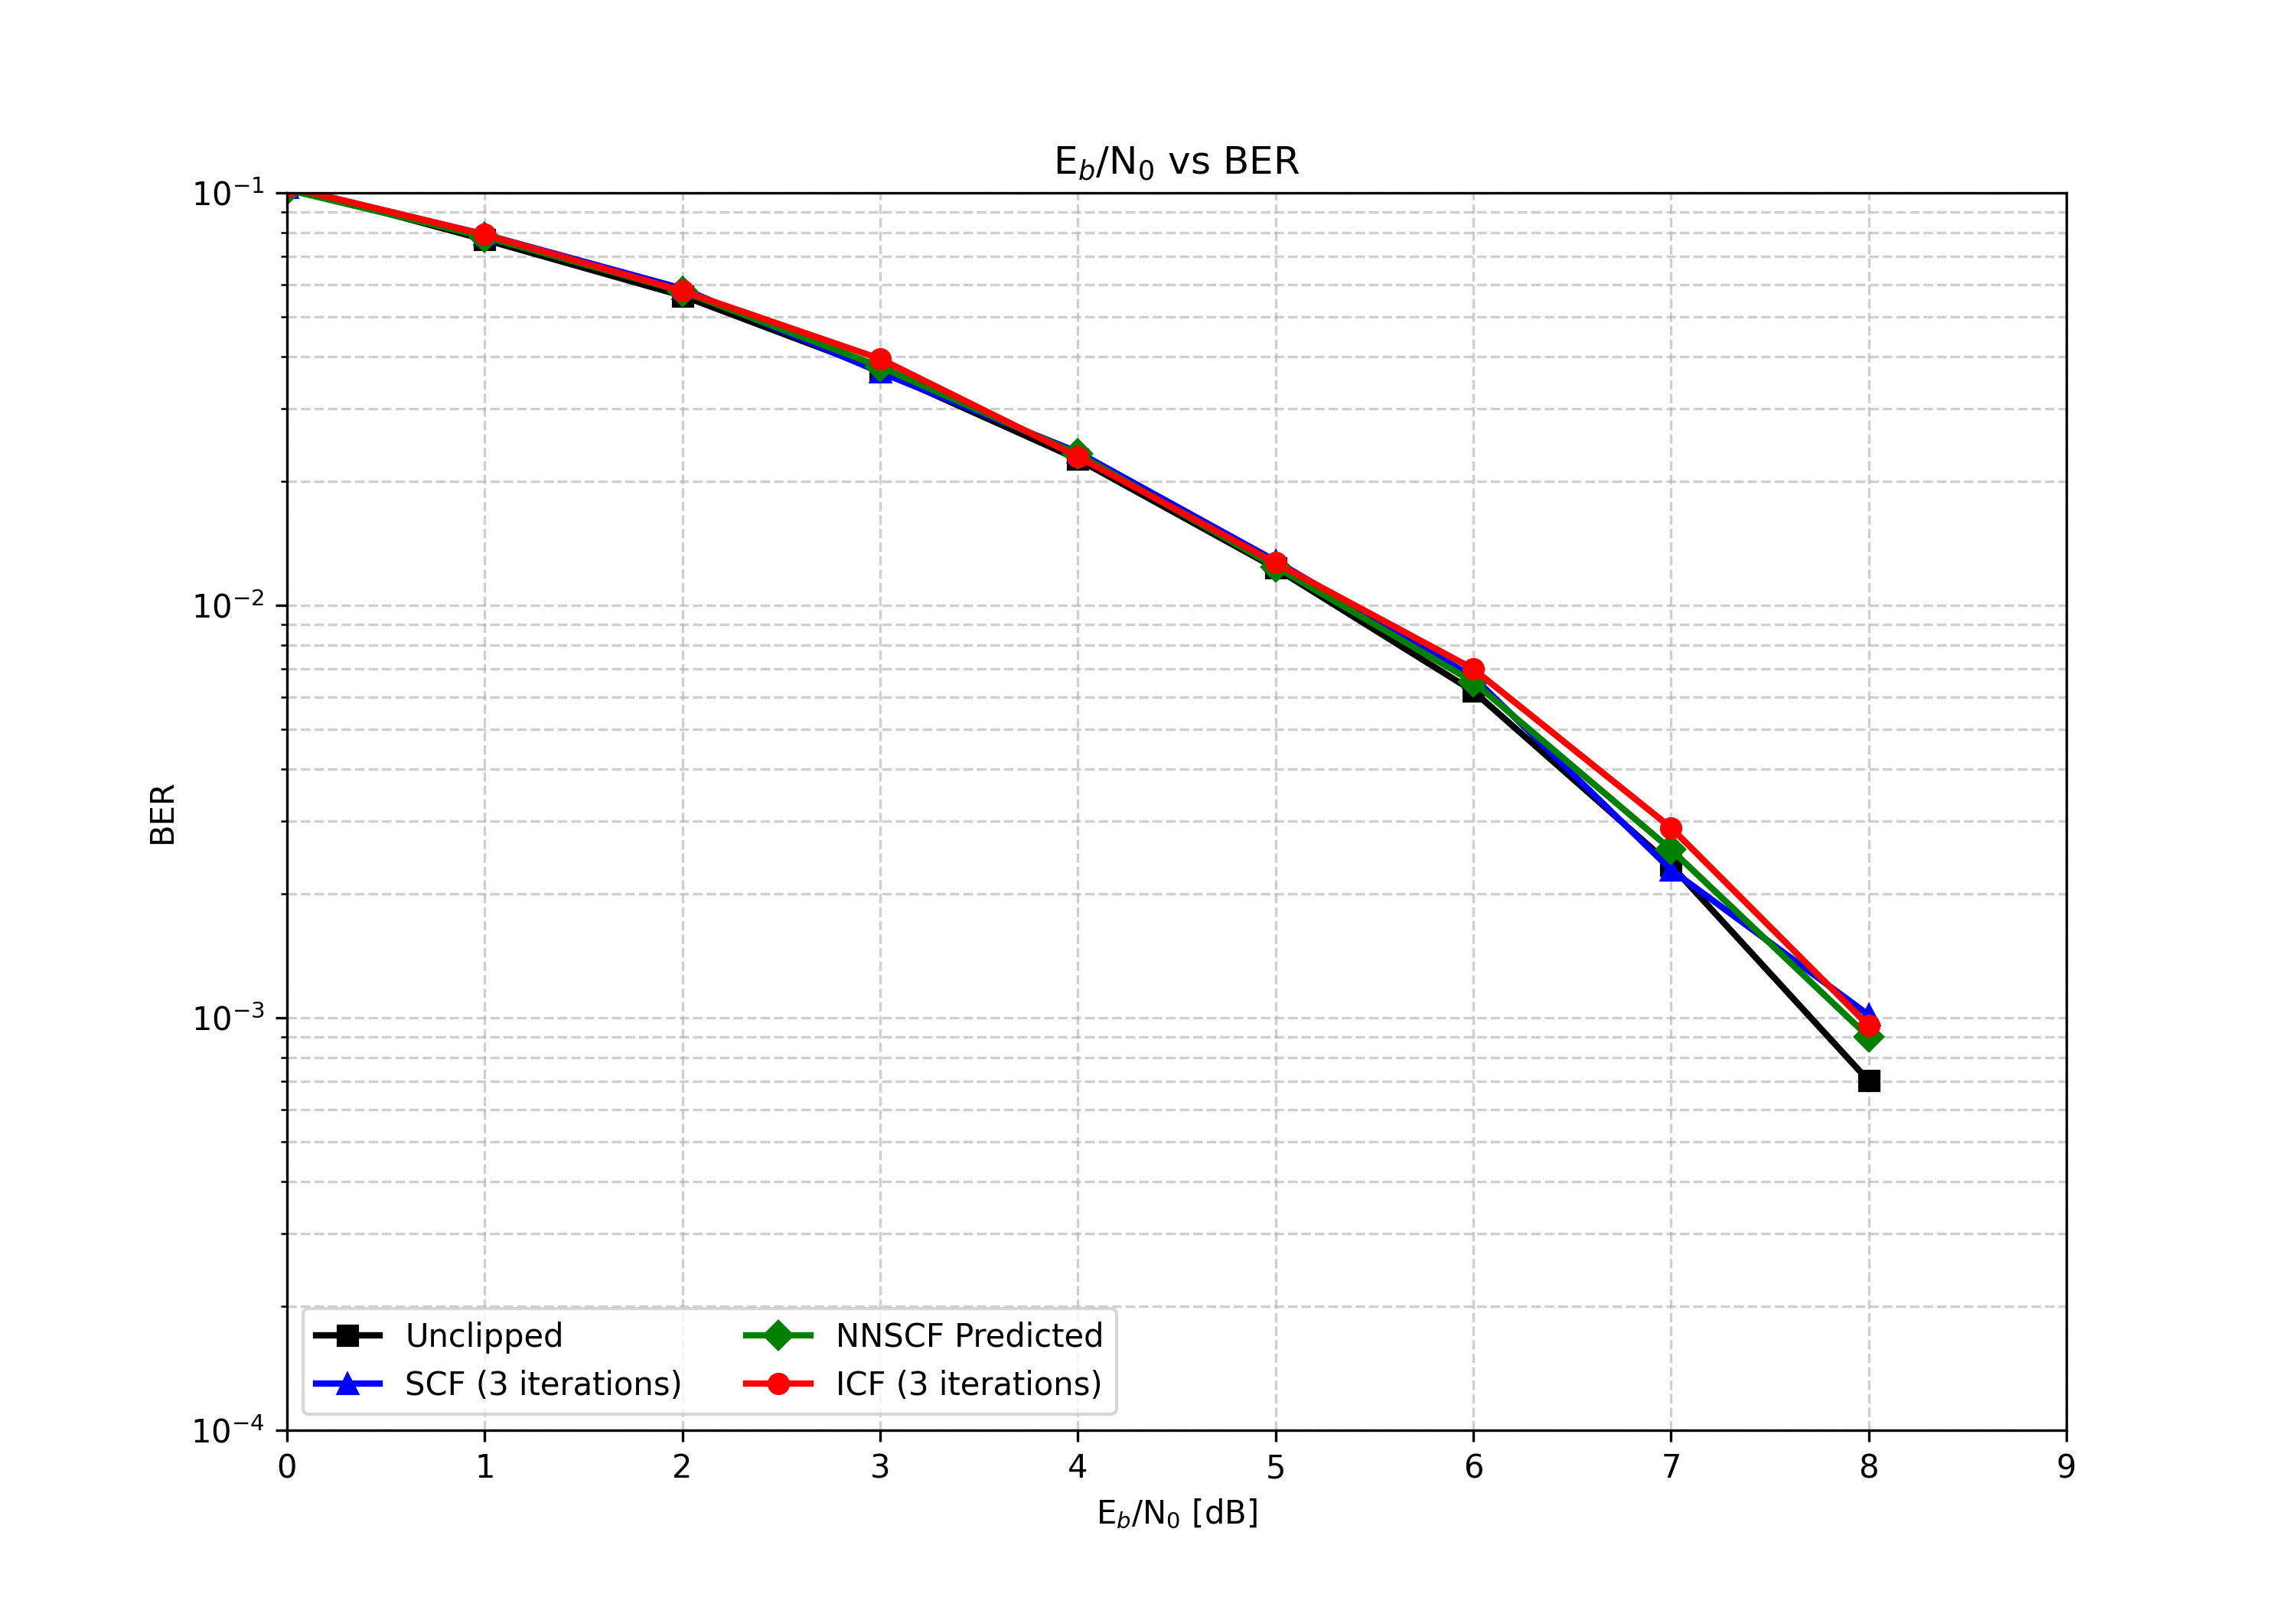
\includegraphics[width=0.96\textwidth]{Figures/NN_SCF/ber_qpsk_reproduced.png}
        \caption{Our simulated results}
        \label{fig:ber_qpsk_reproduced}
    \end{subfigure}
    \caption{Bit Error Rate (BER) comparison over an AWGN channel for QPSK modulation ($N=256$), comparing (a) original results~\cite{sohn2015neural} and (b) our simulated reproduction. The plot evaluates signal reconstruction quality under different peak-limiting frameworks.}
    \label{fig:ber_qpsk_comparison}
\end{figure}

As shown in Figure~\ref{fig:ber_qpsk_comparison}, the BER curves of all techniques for QPSK are virtually identical. The NN-SCF mapper successfully limits the peak power without introducing any additional in-band distortion, tracking the theoretical original OFDM BER down to $10^{-4}$ at $E_b/N_0 = 8$ dB.

Figure~\ref{fig:ber_16qam_comparison} compares the BER performance for the 16-QAM modulation scheme.

\begin{figure}[H]
    \centering
    \begin{subfigure}[b]{0.48\textwidth}
        \centering
        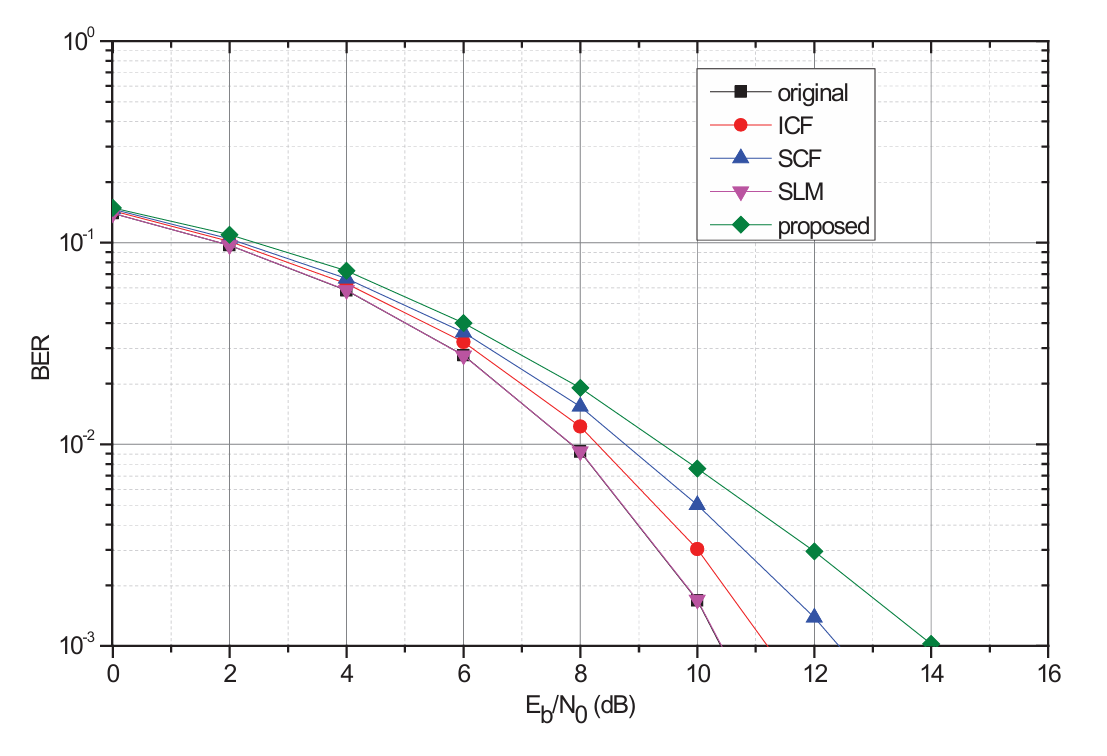
\includegraphics[width=\textwidth]{Figures/NN_SCF/ber_16qam_paper.png}
        \caption{Results from the original paper~\cite{sohn2015neural}}
        \label{fig:ber_16qam_paper}
    \end{subfigure}
    \hfill
    \begin{subfigure}[b]{0.48\textwidth}
        \centering
        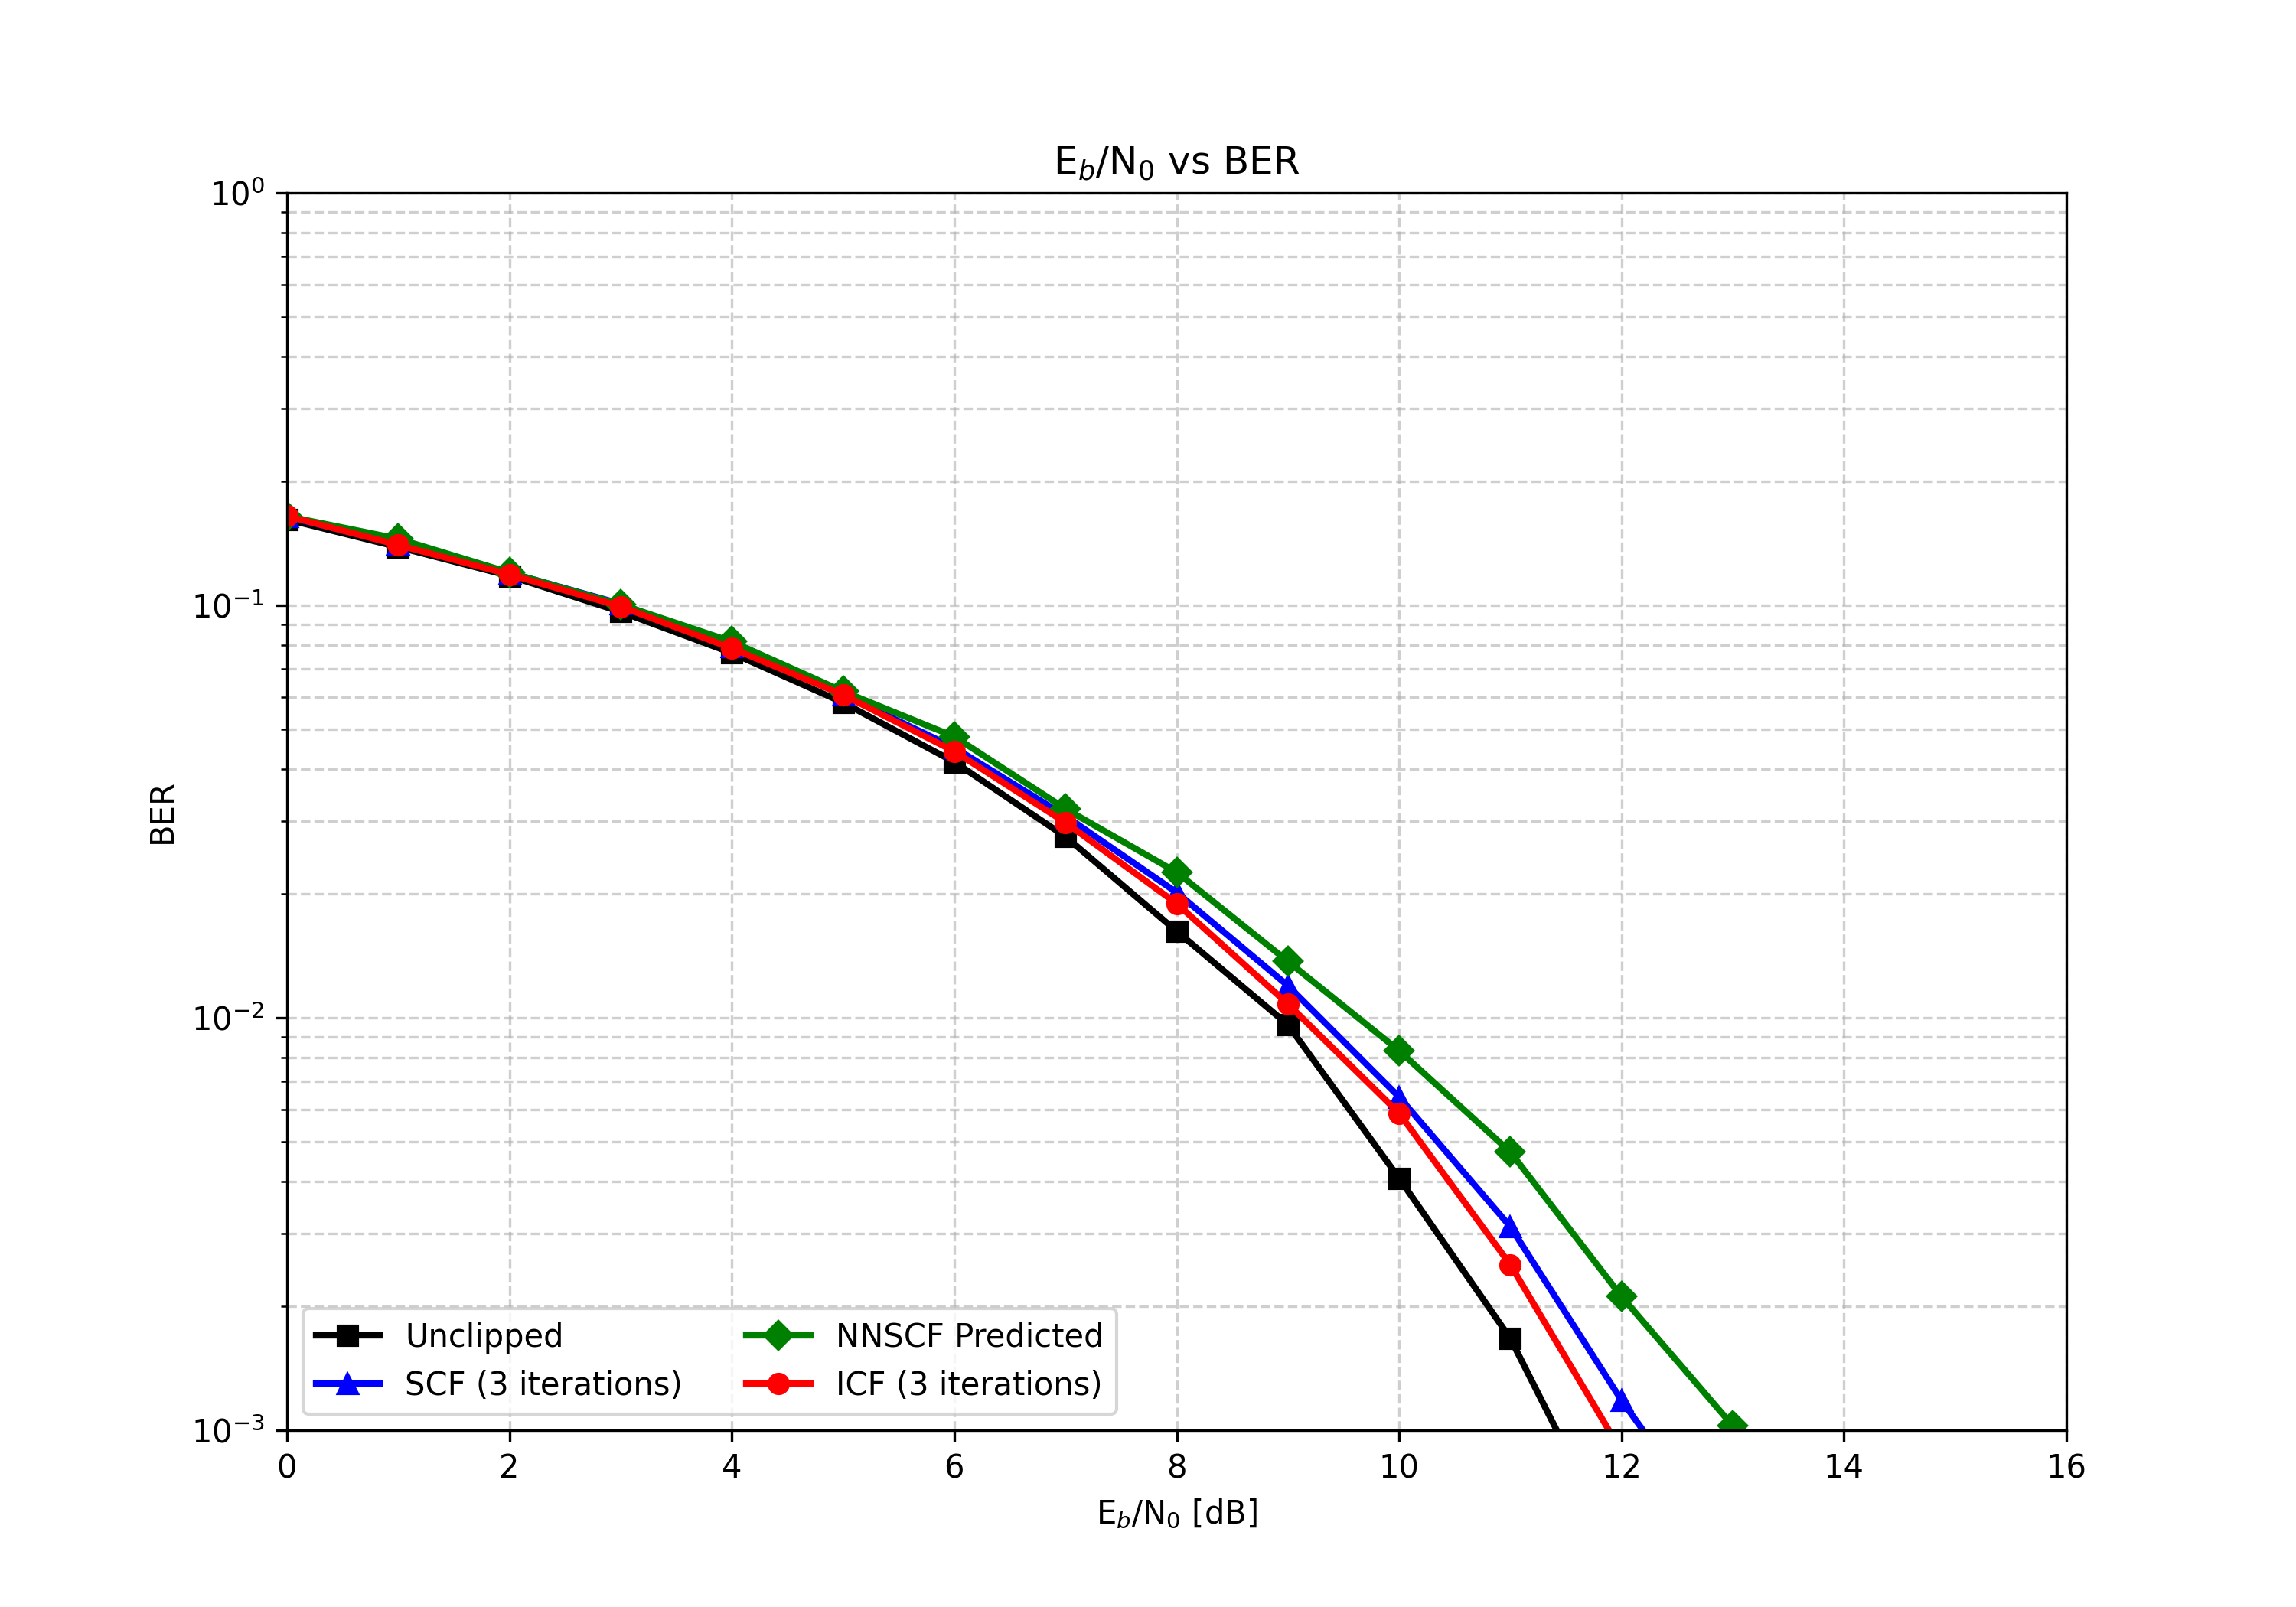
\includegraphics[width=0.96\textwidth]{Figures/NN_SCF/ber_16qam_reproduced.png}
        \caption{Our simulated results}
        \label{fig:ber_16qam_reproduced}
    \end{subfigure}
    \caption{Bit Error Rate (BER) comparison over an AWGN channel for 16-QAM modulation ($N=256$), comparing (a) original results~\cite{sohn2015neural} and (b) our simulated reproduction. The plot highlights the performance gap under higher-order amplitude modulation schemes.}
    \label{fig:ber_16qam_comparison}
\end{figure}

Unlike QPSK, the 16-QAM results reveal a small performance gap. The NN-SCF curves exhibit an SNR penalty of approximately $1.5$ dB at a target BER of $10^{-3}$ compared to classical SCF. This is because 16-QAM utilizes multiple amplitude levels. The increased constellation complexity makes it more difficult for a highly restricted $1\text{--}2\text{--}1\text{--}1$ neural network to map the exact non-linear boundaries, causing minor frequency-domain information loss. However, the system retains a significant complexity advantage over the classical benchmarks.

% ============================================================================
\section{Limitations}
\label{sec:nnscf_limitations}
% ============================================================================

Despite its advantages, several limitations were identified during the implementation:
\begin{itemize}
    \item \textbf{Lack of Spatial Correlation}: The MLP processes the signal sample-by-sample, meaning it cannot capture the temporal correlations introduced by the frequency-domain filter.
    \item \textbf{Configuration Overfitting}: The weights are trained for a specific clipping ratio, modulation scheme, and oversampling rate. Any change in the environment parameters requires retraining.
    \item \textbf{Optimization Constraint}: The PyTorch model had to be trained using the first-order Adam optimizer rather than the second-order Levenberg-Marquardt algorithm proposed in the literature, which restricted training convergence speed.
    \item \textbf{Omitted Parameters}: Several parameters were not given in the research paper, which restricted the ability to exactly replicate its results.
    \item \textbf{Model Capacity}: The highly compact $1\text{--}2\text{--}1\text{--}1$ topology limits mapping accuracy for higher-order constellations like 64-QAM or 256-QAM.
\end{itemize}

% ============================================================================
\section{Future Work}
\label{sec:nnscf_future_work}
% ============================================================================

Future research can address these challenges through the following extensions:
\begin{itemize}
    \item \textbf{Temporal Architectures}: Replacing the MLP with Convolutional Neural Networks (CNNs) or Recurrent Neural Networks (RNNs) to capture sample-to-sample memory and better emulate filter characteristics.
    \item \textbf{Generalized Training}: Training the model across a wide range of clipping ratios and modulation levels to create a single, robust physical-layer block.
    \item \textbf{Subcarrier Scaling}: Expanding the pipeline to evaluate performance and complexity gains on larger subcarrier systems ($N = 1024$ or $2048$).
    \item \textbf{Parameter Optimization}: Having more liberty in choosing the parameters to make sure the mapper gets to the optimum results.
\end{itemize}
